 \documentclass{beamer}

\usetheme{MagdeburgFIN}
\usefonttheme{structurebold}
\usepackage{graphicx}
\usepackage{wrapfig,lipsum}
\usepackage{float}
\usepackage{url}
\usepackage{pdfpages}
\usepackage[ngerman]{babel}
\usepackage[utf8]{inputenc}

\title{Thread Pool in GeckoDB/BOLSTER}
\subtitle{Milestone III: Implementation \& evaluation setup}
\author{Johann Wagner, Johannes Wünsche, Marten Wallewein-Eising, Robert Jenderise}
\date{\today}
\institute{Otto von Guericke University, Magdeburg}

\begin{document}

\begin{frame}[plain]
 \titlepage
\end{frame}

\section[Agenda]{}
	\begin{frame}
	\frametitle{Agenda}
	\tableofcontents
	\end{frame}

\section{Previously...}
\begin{frame}
	\begin{center}
		\huge Previously...
	\end{center}
\end{frame}

\begin{frame}
	\frametitle{Previously on Thread Pool in GeckoDB/BOLSTER}
	\begin{center}
		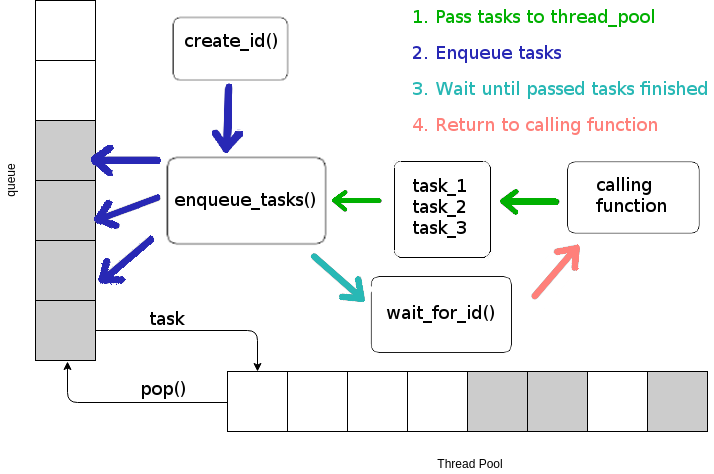
\includegraphics[width=0.9\textwidth]{img/pool_queue.png}
	\end{center}
\end{frame}

\begin{frame}
	\frametitle{Previously on Thread Pool in GeckoDB/BOLSTER}
	\begin{columns}
		\begin{column}{0.48\textwidth}
			\begin{itemize}
				\item Problem: waiting for a task to complete could lead to a
				race condition
				\item This was caused by the uncertainty of a thread\_task
				during transition between the priority queue and the
				thread pool
				\item Solution: slotmap with an atomic counter
			\end{itemize}
		\end{column}
		\begin{column}{0.48\textwidth}
			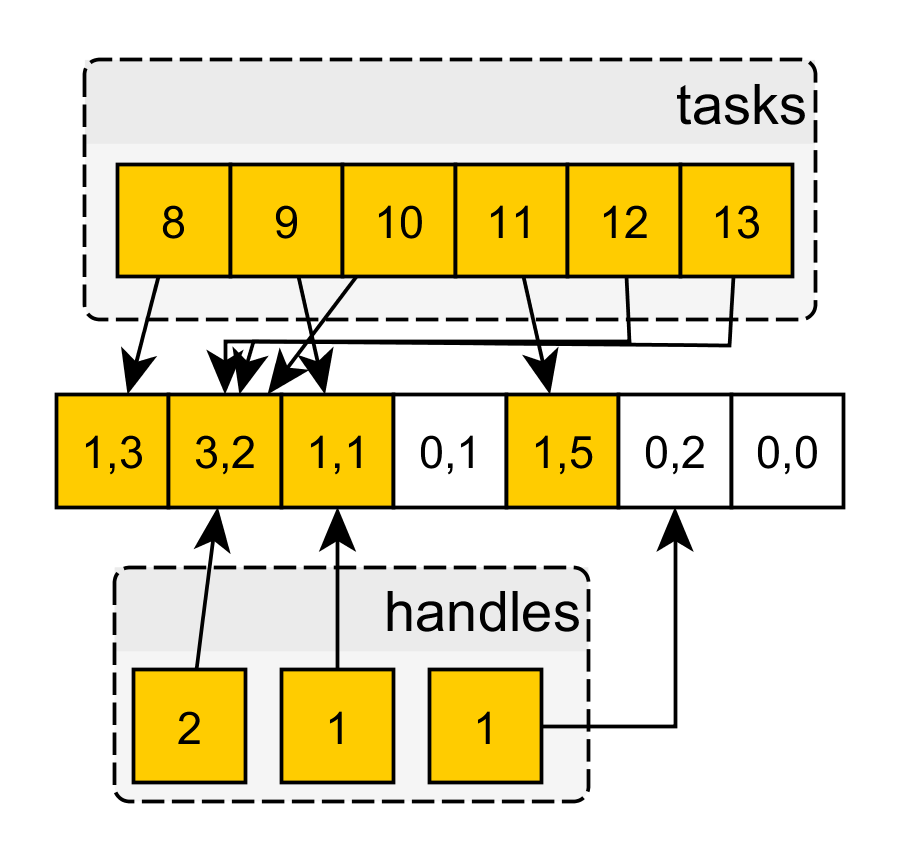
\includegraphics[width=1.0\textwidth]{waitingconcept.png}
		\end{column}
	\end{columns}
\end{frame}

\section{Implementation}
\begin{frame}
	\begin{center}
		\huge Implementation
	\end{center}
\end{frame}

\begin{frame}
	\frametitle{Design of Thread Pool System}
	\begin{center}
		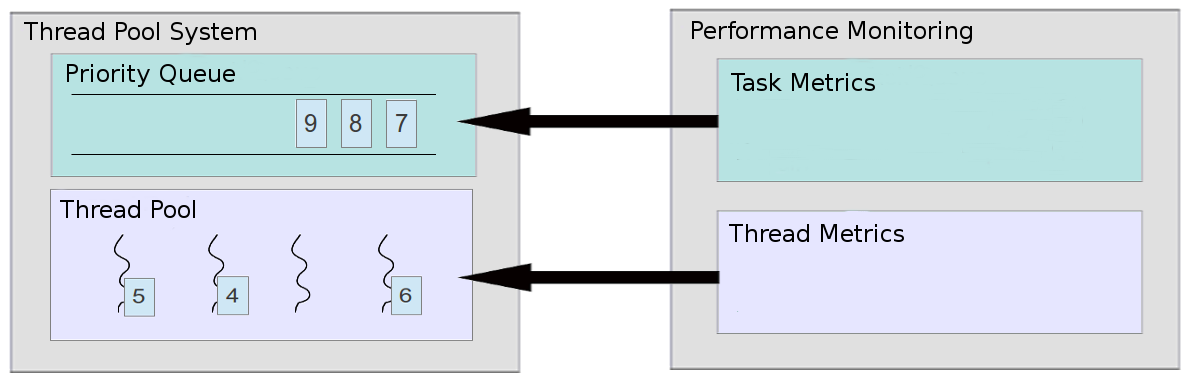
\includegraphics[width=0.9\textwidth]{img/pool_structure.png}
	\end{center}
	\begin{itemize}
		\item Thread pool system contains priority queue and thread pool itself
		\item Performance monitoring as optional, external component
	\end{itemize}
\end{frame}

\begin{frame}
	\frametitle{Implementation}
	We...
	\begin{itemize}
		\item Implemented task enqueueing and execution
		\item Implemented performance monitoring as external component
		\item Added gtest framework to project and wrote tests for pool and queue
		\item Started writing performance tests and measures for comparison against baseline
	\end{itemize}
\end{frame}

\begin{frame}
	\frametitle{Usage Examples}
	\begin{center}
		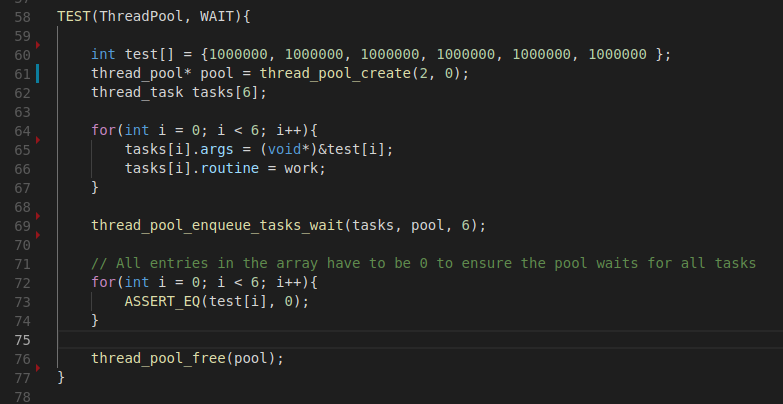
\includegraphics[width=0.95\textwidth]{img/thread_pool_use.png}
	\end{center}
\end{frame}

\begin{frame}
\frametitle{Usage Examples}
\begin{center}
	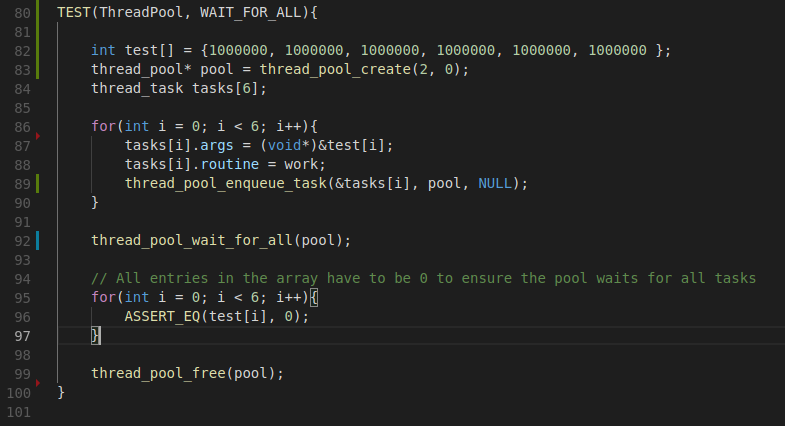
\includegraphics[width=0.95\textwidth]{img/thread_pool_use2.png}
\end{center}
\end{frame}

\begin{frame}
	\frametitle{Open issues}
	\begin{itemize}
		\item GTest still has some problems with c atomics due to itself being implemented in C++
		\item Some race condition may still occur
		\item Check for memory leaks using valgrind
	\end{itemize}
\end{frame}

\section{Evaluation Setup}
\begin{frame}
	\begin{center}
		\huge Evaluation Setup
	\end{center}
\end{frame}

\begin{frame}
	\frametitle{Evaluation Setup}
	\begin{itemize}
		\item Use of geckodb to stress test the thread pool by with BOLSTER primitives
		\item Measure different statistics for tasks, thread and thread pools
		\item Use statistics to determine optimal configurations for different thread pool instances
		\item Time measures are taken with wall clock time
	\end{itemize}
\end{frame}

\begin{frame}
	\frametitle{Task Statistics}
	\begin{center}
		\begin{tabular}{ c c }
			\hline
			\textbf{Statistic name}&\textbf{Description}\\
			\hline
			enqueue\_time & Time when the task was enqueued \\
			execution\_time & Time when the task execution begins \\
			complete\_time & Time when the task execution is finished \\
			\hline
		\end{tabular}
		\label{tab2}
	\end{center}
	\begin{itemize}
		\item Minimize waiting time $(execution\_time - enqueue\_time)$
		\item Evaluate the task setup considering the whole processing time 
	\end{itemize}
\end{frame}

\begin{frame}
	\frametitle{Thread Statistics}
	\begin{center}
		\begin{tabular}{ c c }
			\hline
			\textbf{Statistic name}&\textbf{Description}\\
			\hline
			waiting\_time & Time the thread spend waiting (ns) \\
			busy\_time & Time the thread spend executing tasks (ns)\\
			task\_count & Number of tasks the thread has executed \\
			\hline
		\end{tabular}
		\label{tab3}
	\end{center}
	\begin{itemize}
		\item $waiting\_time$ of threads indicate a good thread pool size
		\item $task\_count$ interesting to number of all completed tasks
	\end{itemize}
\end{frame}

\begin{frame}
	\frametitle{Thread Pool Statistics}
	\begin{center}
		\begin{tabular}{ c c }
			\hline
			\textbf{Statistic name}&\textbf{Description}\\
			\hline
			working\_time & Time the thread pool runs (ns) \\
			task\_complete\_count & Number of completed tasks \\
			task\_enqueued\_count & Number of enqueued tasks \\
			avg\_complete\_time & Average time span from enqueueing until \\
			& execution of tasks \\
			avg\_wait\_time & Average time of tasks spend in the queue \\
			\hline
		\end{tabular}
		\label{tab4}
	\end{center}
	\begin{itemize}
		\item $avg\_wait\_time$ indicates the quality of the chosen thread pool size
	\end{itemize}
\end{frame}

\begin{frame}
	\frametitle{Possible Optimization Opportunities}
	\begin{itemize}
		\item Improve Priority Queue data structure
		\item Change distribution of Wait-Slots
		\item Reduce number of dynamic allocations
		\item Adjust number of threads to increase occupancy
	\end{itemize}
\end{frame}

\section{Paper Progress}
\begin{frame}
	\begin{center}
	\huge Paper Progress \normalsize	
	\end{center}
\end{frame}

\begin{frame}
	\begin{itemize}
		\item Introduction and Preliminaries completed
		\item Implementation described, including our used concepts and basic ideas how to build and operate the pool
		\item Still required are the evaluation (since we still need to
			measure the actual performance), the description of our testing environment and our final conclusion
	\end{itemize}
\end{frame}

\begin{frame}
    \frametitle{Thank you for your attention!}
 	
\includegraphics[width=\textwidth]{img/important.jpg}
\end{frame}

\end{document}
